\documentclass[10pt, compress]{beamer}

\usetheme{m}

\usepackage{booktabs}
\usepackage{xcolor}
\usepackage[scale=2]{ccicons}
\usepackage{listings}
\usepackage{graphicx}

\usepgfplotslibrary{dateplot}

%Colors
\definecolor{light_gray}{HTML}{aaaaaa}

%Commands
\newcommand{\up}[1]{\textsuperscript{\textbf{\textsc{#1}}}}
%\setbeameroption{show notes}
\lstset{language=Java,
                columns=flexible,
  basicstyle={\tiny\ttfamily},
  numberstyle=\tiny\color{gray},
  keywordstyle=\color{orange},
  commentstyle=\color{light_gray},
  stringstyle=\color{orange},
  tabsize=2,
  aboveskip=5pt,
  belowskip=5pt,
}

\title{Conception et développement d’une application d’annotation thématique}
\subtitle{dans l’environnement Gate}
\date{\today}
\author{Charles Follet \and Roland Bary}
\institute{Université de Pau et Pays de l'Adour}

\begin{document}

\maketitle
\begin{frame}[fragile]
	\frametitle{Introduction}
		\begin{itemize}[<+->]
  			\setbeamertemplate{itemize item}[square]
  			\item{Extension du web vers un web dit de données: le web sémantique}
  			\item{Recherche sémantique: activité du web sémantique}
  			\item{Annotation sémantique: Étape du processus de recherche sémantique}
  			\item{Problème: Comment annoter sémantiquement un document texte non-structuré ?}
  			\item{Quelles outils pour l'annotation ?}
  			\item{Quelle approche de conception ?}
  		\end{itemize}
\end{frame}

\begin{frame}[fragile]
  \frametitle{Sommaire}
  \tableofcontents
\end{frame}
%%%%%%%%%%%%%%%%%%%%%%%%%%%%%
%	Cahier des charges		%
%%%%%%%%%%%%%%%%%%%%%%%%%%%%%
\section{Le cahier des charges}
\begin{frame}[fragile]
	\frametitle{Le cahier des charges}
	Contexte: Recherche d'informations sur le Numéraire Carolingien de Georges DEPEYROT.
	\begin{columns}
		\onslide<1>
		\column{.4\linewidth}
			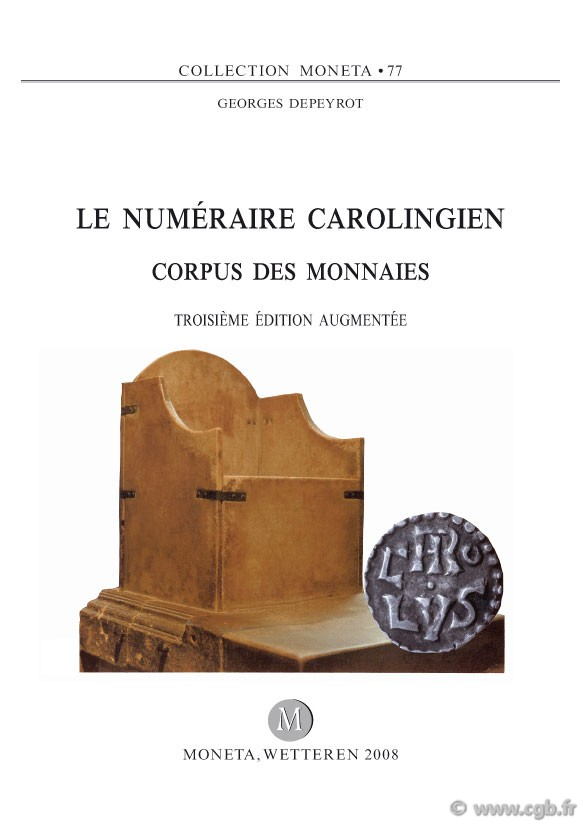
\includegraphics[scale=0.2]{img/depeyrot.jpg}
		\onslide<1>
		\column{.6\linewidth}
		\begin{scriptsize}
			Exemples de recherches possibles:
			\begin{itemize}
				\setbeamertemplate{itemize item}[square]
				\item{Temporelle: Quelles étaient les pièces en circulation de l’an 859 à l’an 865 ?}
				\item{Spatiale: Dans quels ateliers, les pièces de type Obole de Charlemagne ont été produites ?}
				\item{Thématique: Combien d’exemplaires de la monnaie d’or de Charles le Chauve ont été étudiés ?}
			\end{itemize}	
		\end{scriptsize}
	\end{columns}
\end{frame}

\begin{frame}[fragile]
	\frametitle{Le cahier des charges}
	Contexte: Recherche d'informations sur le Numéraire Carolingien de Georges DEPEYROT.
	\begin{columns}
		\onslide<1>
		\column{.4\linewidth}
			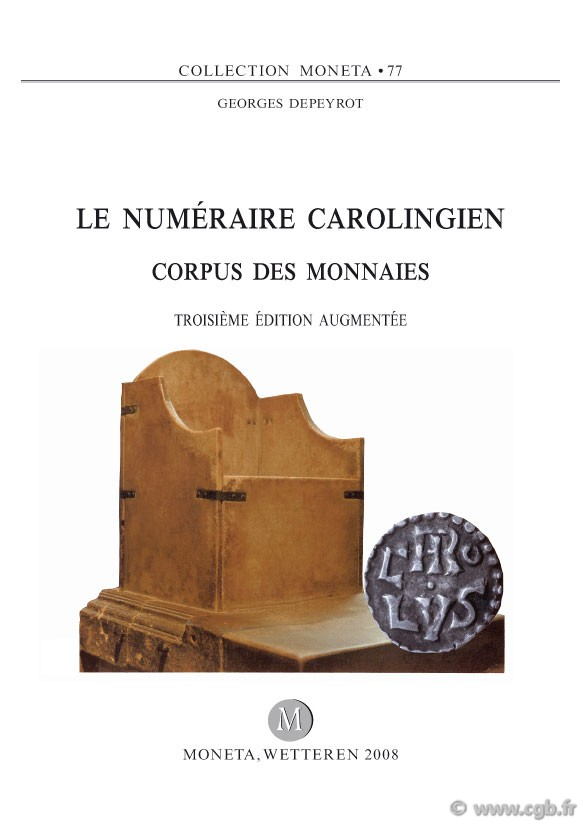
\includegraphics[scale=0.2]{img/depeyrot.jpg}
		\onslide<1>
		\column{.6\linewidth}
		\begin{scriptsize}
			Exemples de recherches possibles:
			\begin{itemize}
				\setbeamertemplate{itemize item}[square]
				\item{Temporelle: Quelles étaient les pièces en circulation de l’an 859 à l’an 865 ?}
				\item{Spatiale: Dans quels ateliers, les pièces de type Obole de Charlemagne ont été produites ?}
				\item{Thématique: Combien d’exemplaires de la monnaie d’or de Charles le Chauve ont été étudiés ?}
			\end{itemize}	
		\end{scriptsize}
	\end{columns}
	Solution: Utilisation d'un outil de Traitement automatique du langage.
\end{frame}

\begin{frame}[fragile]
	\frametitle{Le cahier des charges}
	Caractéristiques du projets:\\
	\begin{itemize}[<+->]
	\setbeamertemplate{itemize item}[square]
		\item{apprentissage et compréhension du domaine considéré}
		\item{étude des principes d'annotation de documents}
		\item{développement d'une chaîne d'annotation dans GATE}
		\item{mise en place d'une interface web de visualisation des résultats}
	\end{itemize}
\end{frame}

\begin{frame}[fragile]
	\frametitle{Le cahier des charges}
	Scénario attendu:
	\begin{scriptsize}
	Texte en entrée de traitement
	\end{scriptsize}
	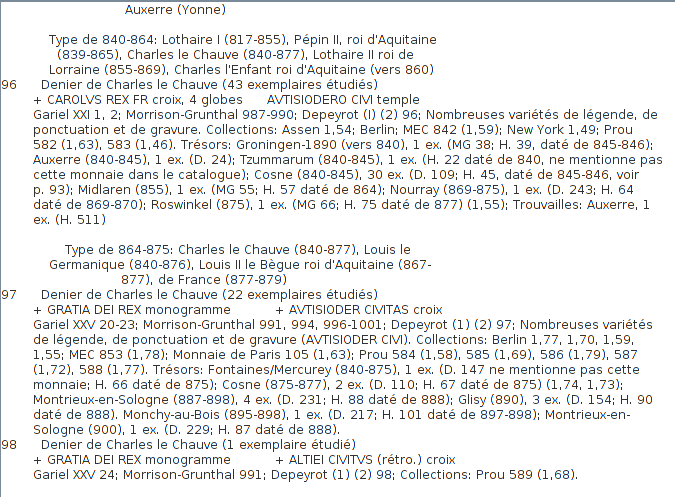
\includegraphics[scale=0.3]{img/beforean.png}
\end{frame}

\begin{frame}[fragile]
	\frametitle{Le cahier des charges}
	Scénario attendu:
	\begin{scriptsize}
	Texte en sortie de traitement
	\end{scriptsize}
	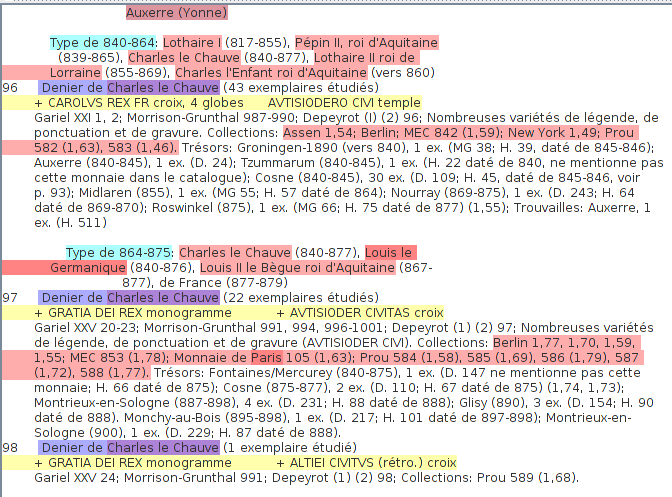
\includegraphics[scale=0.3]{img/afteran.png}
\end{frame}

%%%%%%%%%%%%%%%%%%%%%%%%%%%%%
%	Cadre d'analyse			%
%%%%%%%%%%%%%%%%%%%%%%%%%%%%%
\section{Cadre d'analyse}
\subsection{L'environnement GATE}
\begin{frame}[fragile]
\frametitle{Cadre d'analyse - L'outil GATE}
\begin{columns}
	\onslide<1>
	\column{.6\linewidth}
	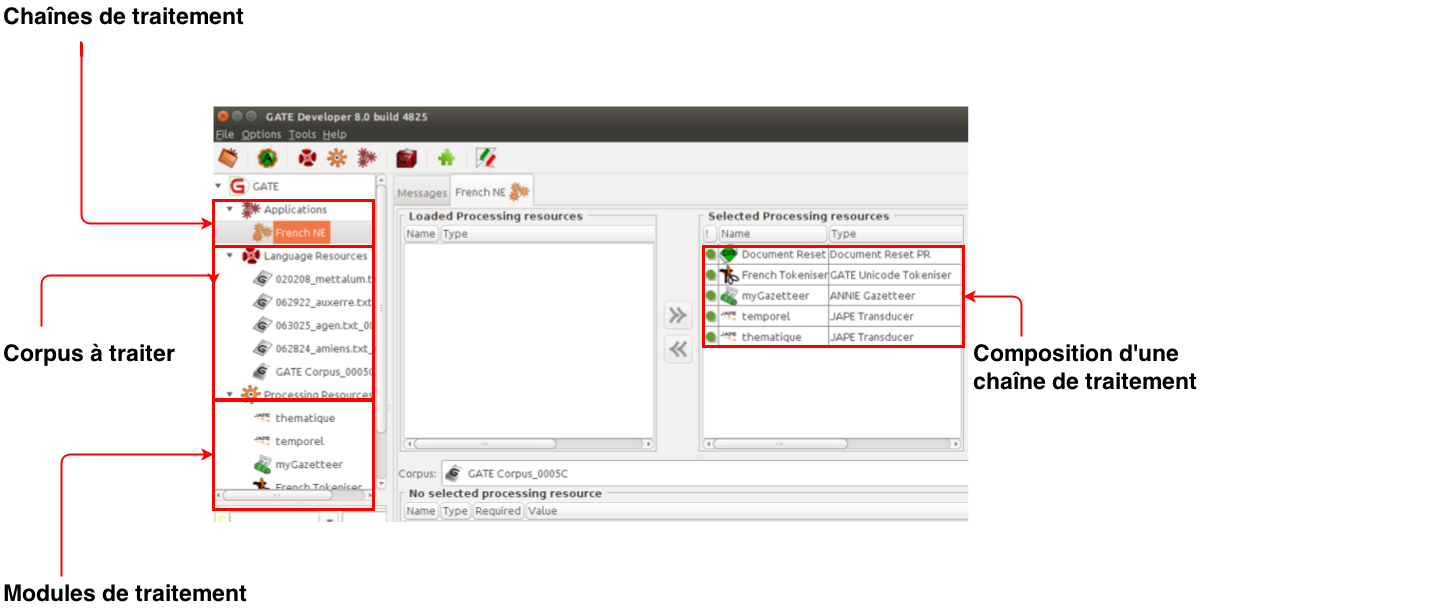
\includegraphics[scale=0.190]{img/gatePresent.png} 
	\onslide<1>
	\column{.4\linewidth}
	\begin{scriptsize}
		\setbeamertemplate{itemize item}[square]
	\begin{itemize}
		\item{Outil de traitement automatique du langage (en JAVA).}
		\item{Université de Sheffield 1995.}
		\item{Principe: Chaîne de traitement (Pipeline).}
		\item{Plusieurs modules dans un pipeline.}
		\item{ANNIE: Pipeline par défaut pouvant servir de chaîne de départ}
	\end{itemize}
	\end{scriptsize}
\end{columns}
\end{frame}

\begin{frame}[fragile]
\frametitle{Cadre d'analyse - L'outil GATE}
\begin{columns}
	\onslide<1>
	\column{.6\linewidth}
	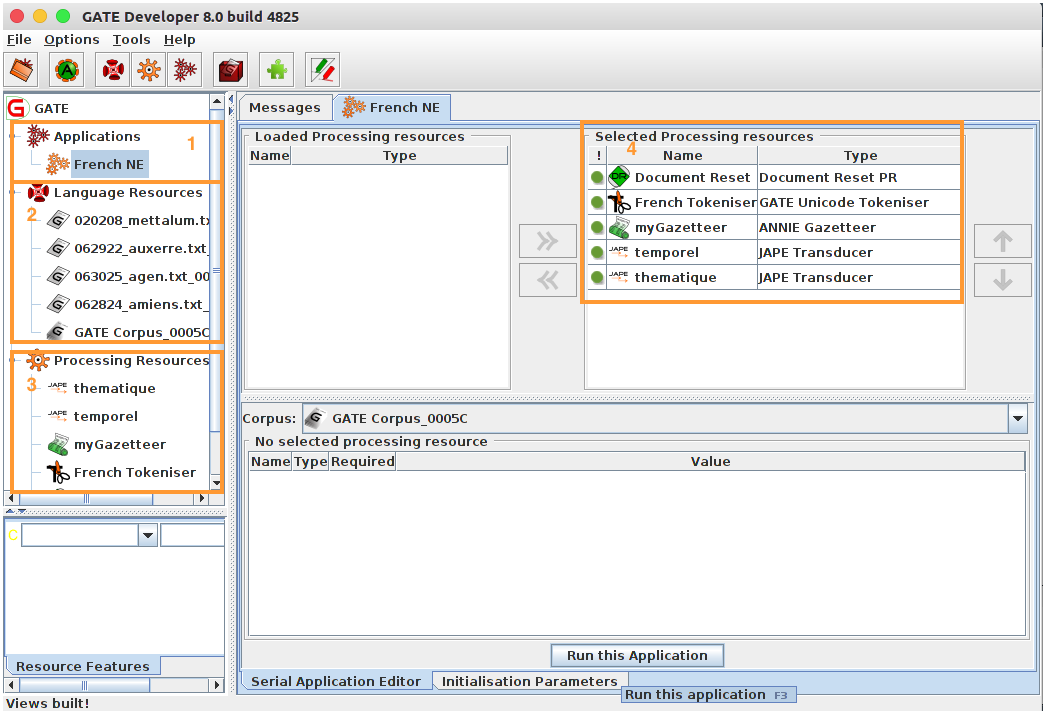
\includegraphics[scale=0.2]{img/gateMod.png} 
	\onslide<1>
	\column{.3\linewidth}
	\begin{scriptsize}
		\setbeamertemplate{itemize item}[square]
	\begin{itemize}	
		\item{1- Chaîne de traitement}
		\item{2- Textes et corpus à traiter}
		\item{3- Modules d'annotation}
		\item{4- Composition d'une chaîne de traitement}
	\end{itemize}
	\end{scriptsize}
\end{columns}
\end{frame}

\begin{frame}[fragile]
\frametitle{Cadre d'analyse - L'outil GATE}
\begin{itemize}
\setbeamertemplate{itemize item}[square]
	\item{Exemple de la chaîne de traitement ANNIE}
\end{itemize}
	\begin{columns}
	\onslide<1>
	\column{.6\linewidth}
		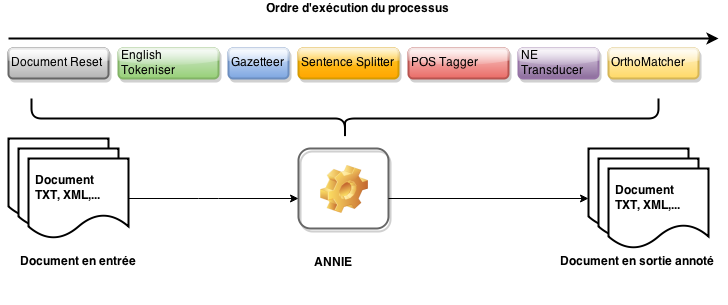
\includegraphics[scale=0.2]{img/annieChaine.png} 
	\onslide<1>
	\column{.3\linewidth}
	\begin{scriptsize}
		\begin{itemize}
			\setbeamertemplate{itemize item}[square]
			\item{Module Gazetter: Identification des noms d'entité dans le texte, sur la base d'un gazetier}
			\item{Module NE Transducer: Repérage d'entités nommées inconnues en fonction de modèles d'extraction écrits en langage JAPE}
		\end{itemize}
	\end{scriptsize}
	\end{columns}
\end{frame}

\subsection{Les Gazetiers}
\begin{frame}[fragile]
\frametitle{Cadre d'analyse - Gazetiers}
\begin{columns}
	\onslide<1>
	\column{.6\linewidth}
		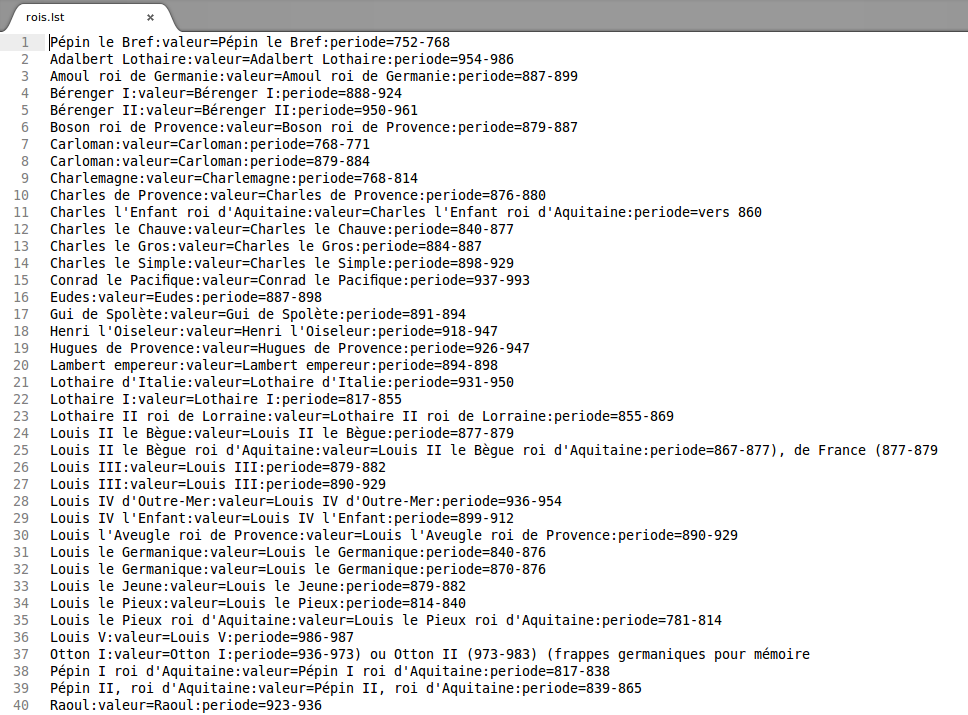
\includegraphics[scale=0.2]{img/Gaz.png} 
	\onslide<1>
	\column{.4\linewidth}
		\begin{scriptsize}
		\begin{itemize}
			\setbeamertemplate{itemize item}[square]
			\item{liste de noms d'entités (Villes, métiers,etc)}
			\item{permettant un repérage d’occurrences dans un texte}
			\item{possibilité d'associer des caractéristiques a chaque nom d'entité (séparateurs)}
			\item{Dans Gate: MajorType, MinorType}
		\end{itemize}
		\end{scriptsize}
	\end{columns}
\end{frame}

\subsection{Le formalisme JAPE}
\begin{frame}[fragile]
\frametitle{Cadre d'analyse - Le formalisme JAPE}
\begin{columns}
	\onslide<1>
	\column{.6\linewidth}
	\begin{scriptsize}
\begin{lstlisting}
Phase: pourcent
Input: Lookup Token
Options: control = appelt
/**************************** MACROS */
Macro: AMOUNT_NUMBER
(({Token.kind == number}
(
({Token.string == ","} | {Token.string == "."})
{Token.kind == number}
)?
({Token.string == "-"}{Token.kind == number})?))
Macro: PERCENT(
{Token.string == "%"} |
{Token.string == "pourcent"}|
({Token.string == "pour"}{Token.string == "cent"})14)
Macro: LIAISON_PERCENT_DE_ET(
{Token.string == "de"}|
{Token.string == "et"}|
{Token.string == ","})
/***************************** Regle */
Rule: Percent_number
/***************************** LHS */
(((AMOUNT_NUMBER)
({Token.string == "à"})
)?(AMOUNT_NUMBER)(PERCENT))
:pourcent
/***************************** RHS */ 
-->:pourcent.Percent = 
{Kind="pourcent",Rule="Percent_number"}
\end{lstlisting}
\end{scriptsize}
	\onslide<1>
	\column{.4\linewidth}
	\begin{scriptsize}
	\begin{itemize}
	\setbeamertemplate{itemize item}[square]
	
	\item{Règles JAPE en deux blocs}
	\item{Partie gauche (LHS): définition d'un motif d'annotation à repérer}
	\item{Partie droite (RHS): Opérations sur un motif (Code JAVA éventuel)}
	\item{Utilisation d'un système de Macros}
	\end{itemize}
	
	\end{scriptsize}
\end{columns}
\end{frame}
%%%%%%%%%%%%%%%%%%%%%%%%%%%%
%   Structure du numeraire %
%%%%%%%%%%%%%%%%%%%%%%%%%%%%
\section{Structure du numéraire}
\begin{frame}[fragile]
\frametitle{Exemple}
\begin{scriptsize}
Agen (Lot-et-Garonne)\\~\\

Type de 793/4-812: Charlemagne (768-814)\\
Denier de Charlemagne (24 exemplaires étudiés)\\
+ CARLVS REX FR croix~~~~~~~ + AGINNO monogramme\\
Gariel XXII 26; Morrison-Grunthal 177-179; Depeyrot (1) (2) 1; Collections: Berlin 1,64, 1,45;\\
Bruxelles 1,25, 1,25; Charleville-Mézières 1,56; Copenhague 1,31; Garett 1,73; Grenoble; MEC 735 \\
(1,57), 736 (1,24); Monnaie de Paris 88 (1,55); New York 1,64, 1,57; Prou 792 (1,36), 793 (1,60), \\
794 (1,50) Trésors: Biebrich (790-814), 2 ex. (MG 11, Vôlkers, p. 182) (1,60); Ibersheim (814), 1 ex. \\
(MG 13, Vôlkers, p. 186) (1,64); Dorestad (822), 4 ex. (MG 18, Vôlkers, p. 139; H. 7) (1,35);\\
Trouvailles: Bolsward, 1 ex. (H. 528) (1,26).
\end{scriptsize}
\note{Le Numeraire est organisé en atelier, un atelier fabrique une ou plusieurs monnaies. On voit ici l'atelier d'Agen. Nous allons détailler tous les éléments à l'écran}
\end{frame}

\begin{frame}[fragile]
  \frametitle{L'atelier}
  \begin{scriptsize}
\textbf{Agen (Lot-et-Garonne)}\\~\\
\textcolor{light_gray}{
Type de 793/4-812: Charlemagne (768-814)\\
Denier de Charlemagne (24 exemplaires étudiés)\\
+ CARLVS REX FR croix~~~~~~~ + AGINNO monogramme\\
Gariel XXII 26; Morrison-Grunthal 177-179; Depeyrot (1) (2) 1; Collections: Berlin 1,64, 1,45; \\
Bruxelles 1,25, 1,25; Charleville-Mézières 1,56; Copenhague 1,31; Garett 1,73; Grenoble; MEC 735 \\
(1,57), 736 (1,24); Monnaie de Paris 88 (1,55); New York 1,64, 1,57; Prou 792 (1,36), 793 (1,60), \\
794 (1,50) Trésors: Biebrich (790-814), 2 ex. (MG 11, Vôlkers, p. 182) (1,60); Ibersheim (814), 1 ex. \\
(MG 13, Vôlkers, p. 186) (1,64); Dorestad (822), 4 ex. (MG 18, Vôlkers, p. 139; H. 7) (1,35); \\Trouvailles: Bolsward, 1 ex. (H. 528) (1,26).
} 
\end{scriptsize}
    
    \note{Forme : Ville (Dpt|Pays)?}
\end{frame}

\begin{frame}[fragile]
  \frametitle{Le type}
  \begin{scriptsize}
\textcolor{light_gray}{Agen (Lot-et-Garonne)}\\~\\

\textbf{Type de 793/4-812: Charlemagne (768-814)}\\
\textcolor{light_gray}{
Denier de Charlemagne (24 exemplaires étudiés)\\
+ CARLVS REX FR croix~~~~~~~ + AGINNO monogramme\\
Gariel XXII 26; Morrison-Grunthal 177-179; Depeyrot (1) (2) 1; Collections: Berlin 1,64, 1,45; \\
Bruxelles 1,25, 1,25; Charleville-Mézières 1,56; Copenhague 1,31; Garett 1,73; Grenoble; MEC 735 \\
(1,57), 736 (1,24); Monnaie de Paris 88 (1,55); New York 1,64, 1,57; Prou 792 (1,36), 793 (1,60), \\
794 (1,50) Trésors: Biebrich (790-814), 2 ex. (MG 11, Vôlkers, p. 182) (1,60); Ibersheim (814), 1 ex. \\
(MG 13, Vôlkers, p. 186) (1,64); Dorestad (822), 4 ex. (MG 18, Vôlkers, p. 139; H. 7) (1,35); \\Trouvailles: Bolsward, 1 ex. (H. 528) (1,26).
} 
    \end{scriptsize}
    
    \note{Forme : Perdiode(souverains)+}
\end{frame}

\begin{frame}[fragile]
  \frametitle{La nature}
  \begin{scriptsize}
\textcolor{light_gray}{Agen (Lot-et-Garonne)}\\~\\

\textcolor{light_gray}{Type de 793/4-812: Charlemagne (768-814)}\\

\textbf{Denier de Charlemagne (24 exemplaires étudiés)}\\
\textcolor{light_gray}{
+ CARLVS REX FR croix~~~~~~~ + AGINNO monogramme\\
Gariel XXII 26; Morrison-Grunthal 177-179; Depeyrot (1) (2) 1; Collections: Berlin 1,64, 1,45; \\
Bruxelles 1,25, 1,25; Charleville-Mézières 1,56; Copenhague 1,31; Garett 1,73; Grenoble; MEC 735 \\
(1,57), 736 (1,24); Monnaie de Paris 88 (1,55); New York 1,64, 1,57; Prou 792 (1,36), 793 (1,60), \\
794 (1,50) Trésors: Biebrich (790-814), 2 ex. (MG 11, Vôlkers, p. 182) (1,60); Ibersheim (814), 1 ex. \\
(MG 13, Vôlkers, p. 186) (1,64); Dorestad (822), 4 ex. (MG 18, Vôlkers, p. 139; H. 7) (1,35); \\Trouvailles: Bolsward, 1 ex. (H. 528) (1,26).
} 
    \end{scriptsize}
        \note{Forme : Denier, Obole, ... + NOM SOUVERAIN}
\end{frame}

\begin{frame}[fragile]
  \frametitle{La légende}
  \begin{scriptsize}
\textcolor{light_gray}{Agen (Lot-et-Garonne)}\\~\\

\textcolor{light_gray}{Type de 793/4-812: Charlemagne (768-814)\\
Denier de Charlemagne (24 exemplaires étudiés)}\\

\textbf{+ CARLVS REX FR croix~~~~~~~ + AGINNO monogramme}\\
\textcolor{light_gray}{
Gariel XXII 26; Morrison-Grunthal 177-179; Depeyrot (1) (2) 1; Collections: Berlin 1,64, 1,45; \\
Bruxelles 1,25, 1,25; Charleville-Mézières 1,56; Copenhague 1,31; Garett 1,73; Grenoble; MEC 735 \\
(1,57), 736 (1,24); Monnaie de Paris 88 (1,55); New York 1,64, 1,57; Prou 792 (1,36), 793 (1,60), \\
794 (1,50) Trésors: Biebrich (790-814), 2 ex. (MG 11, Vôlkers, p. 182) (1,60); Ibersheim (814), 1 ex. \\
(MG 13, Vôlkers, p. 186) (1,64); Dorestad (822), 4 ex. (MG 18, Vôlkers, p. 139; H. 7) (1,35); \\
Trouvailles: Bolsward, 1 ex. (H. 528) (1,26).
} 
    \end{scriptsize}
        \note{Forme :+?LEG droit SPACE  +?LEG revers}
\end{frame}

\begin{frame}[fragile]
  \frametitle{Les collections}
  \begin{scriptsize}
\textcolor{light_gray}{Agen (Lot-et-Garonne)}\\~\\

\textcolor{light_gray}{
Type de 793/4-812: Charlemagne (768-814)\\
Denier de Charlemagne (24 exemplaires étudiés)\\
+ CARLVS REX FR croix~~~~~~~ + AGINNO monogramme
}\\
\textcolor{light_gray}{
Gariel XXII 26; Morrison-Grunthal 177-179; Depeyrot (1) (2) 1; }\textbf{Collections: Berlin 1,64, 1,45; \\
Bruxelles 1,25, 1,25; Charleville-Mézières 1,56; Copenhague 1,31; Garett 1,73; Grenoble; MEC 735 \\
(1,57), 736 (1,24); Monnaie de Paris 88 (1,55); New York 1,64, 1,57; Prou 792 (1,36), 793 (1,60), \\
794 (1,50) }\textcolor{light_gray}{Trésors: Biebrich (790-814), 2 ex. (MG 11, Vôlkers, p. 182) (1,60); Ibersheim (814), 1 ex. \\(MG 13, Vôlkers, p. 186) (1,64); Dorestad (822), 4 ex. (MG 18, Vôlkers, p. 139; H. 7) (1,35); \\Trouvailles: Bolsward, 1 ex. (H. 528) (1,26).
} 
    \end{scriptsize}
\end{frame}

\begin{frame}[fragile]
  \frametitle{Les trésors}
  \begin{scriptsize}
\textcolor{light_gray}{Agen (Lot-et-Garonne)}\\~\\

\textcolor{light_gray}{
Type de 793/4-812: Charlemagne (768-814)\\
Denier de Charlemagne (24 exemplaires étudiés)\\
+ CARLVS REX FR croix~~~~~~~ + AGINNO monogramme
}\\
\textcolor{light_gray}{
Gariel XXII 26; Morrison-Grunthal 177-179; Depeyrot (1) (2) 1;
Collections: Berlin 1,64, 1,45; \\
Bruxelles 1,25, 1,25; Charleville-Mézières 1,56; Copenhague 1,31; Garett 1,73; Grenoble; MEC 735 \\
(1,57), 736 (1,24); Monnaie de Paris 88 (1,55); New York 1,64, 1,57; Prou 792 (1,36), 793 (1,60), \\
794 (1,50) }\textbf{Trésors: Biebrich (790-814), 2 ex. (MG 11, Vôlkers, p. 182) (1,60); Ibersheim (814), 1 ex. \\
(MG 13, Vôlkers, p. 186) (1,64); Dorestad (822), 4 ex. (MG 18, Vôlkers, p. 139; H. 7) (1,35); }\\
\textcolor{light_gray}{
Trouvailles: Bolsward, 1 ex. (H. 528) (1,26).
} 
    \end{scriptsize}
\end{frame}

\begin{frame}[fragile]
  \frametitle{Les trouvailles}
  \begin{scriptsize}
\textcolor{light_gray}{Agen (Lot-et-Garonne)}\\~\\

\textcolor{light_gray}{
Type de 793/4-812: Charlemagne (768-814)\\
Denier de Charlemagne (24 exemplaires étudiés)\\
+ CARLVS REX FR croix~~~~~~~ + AGINNO monogramme
}\\
\textcolor{light_gray}{
Gariel XXII 26; Morrison-Grunthal 177-179; Depeyrot (1) (2) 1;
Collections: Berlin 1,64, 1,45; \\
Bruxelles 1,25, 1,25; Charleville-Mézières 1,56; Copenhague 1,31; Garett 1,73; Grenoble; MEC 735 \\
(1,57), 736 (1,24); Monnaie de Paris 88 (1,55); New York 1,64, 1,57; Prou 792 (1,36), 793 (1,60), \\
794 (1,50) Trésors: Biebrich (790-814), 2 ex. (MG 11, Vôlkers, p. 182) (1,60); Ibersheim (814), 1 ex. \\
(MG 13, Vôlkers, p. 186) (1,64); Dorestad (822), 4 ex. (MG 18, Vôlkers, p. 139; H. 7) (1,35); }\\
\textbf{Trouvailles: Bolsward, 1 ex. (H. 528) (1,26).}
    \end{scriptsize}
\end{frame}

\begin{frame}[fragile]
  \frametitle{Résumé}
  \begin{scriptsize}
Agen (Lot-et-Garonne)\alert{\up{Atelier}}\\~\\
Type de 793/4-812: Charlemagne (768-814)\alert{\up{Type}}\\
Denier de Charlemagne (24 exemplaires étudiés)\alert{\up{Nature}}\\
+ CARLVS REX FR croix~~~~~~~ + AGINNO monogramme\alert{\up{Légende}}\\
Gariel XXII 26; Morrison-Grunthal 177-179; Depeyrot (1) (2) 1;
Collections: Berlin 1,64, 1,45; \\
Bruxelles 1,25, 1,25; Charleville-Mézières 1,56; Copenhague 1,31; Garett 1,73; Grenoble; MEC 735 \\
(1,57), 736 (1,24); Monnaie de Paris 88 (1,55); New York 1,64, 1,57; Prou 792 (1,36), 793 (1,60), \\
794 (1,50)\alert{\up{Collections}} Trésors: Biebrich (790-814), 2 ex. (MG 11, Vôlkers, p. 182) (1,60); Ibersheim (814), 1 ex. \\
(MG 13, Vôlkers, p. 186) (1,64); Dorestad (822), 4 ex. (MG 18, Vôlkers, p. 139; H. 7) (1,35);\alert{\up{Trésors}} \\
Trouvailles: Bolsward, 1 ex. (H. 528) (1,26)\alert{\up{Trouvailles}}.
    \end{scriptsize}
    \note{Nous avons définis toutes les annotations susceptible d’apparaître, nous allons voir dans la partie suivante les méthodes d’annotation à notre disposition}
\end{frame}

\section{Annotations}
\begin{frame}[fragile,t]
\setbeamercovered{transparent}
  \frametitle{Deux façons d'annoter}
 \begin{columns}[t]
 \onslide<1>
  \begin{column}{.5\linewidth}
    {\large \textsc{\alert{Gazetier}}}\\
    \textbf{liste} de valeurs.\\~\\
\begin{scriptsize}
    \begin{itemize}
    \item Type de 754/5-768
    \item Type de 768-771
    \item Type de 771-793/4
    \item Type de 793/4-812
    \item Type de 812-814
    \item ...
    \end{itemize}
\end{scriptsize}
  \end{column}
  \onslide<2>
  \begin{column}{.5\linewidth}
    {\large \textsc{\alert{Règle JAPE}}}\\
    \textbf{règle} basée sur une expression régulière.\\
    \begin{lstlisting}
Macro: CHAINE_DEBUT
(
    ({Token.string =="Type"})({SpaceToken})
    ({Token.string =="de"})({SpaceToken})
)

// Exemple : Type de 758/9-762
Rule: PeriodeEmissionRule
(
    CHAINE_DEBUT ({Periode}):p
):PeriodeEmission
-->:PeriodeEmission.PeriodeEmission = {
 	Kind = "PeriodeEmission" ,
 	D1 = :p.Periode.D1, D2 = :p.Periode.D2
}
\end{lstlisting}
\end{column}
 \end{columns}  
 \note{Un gazetier est une liste de données qui recense toutes les occurrences possibles d'un élément. Par exemple ici, on pourrai constituer un gazetier contenant toutes les périodes de l'ouvrage.\\
 Une règle JAPE est une formule basée sur les expression régulières qui permet de définir l'allure générale d'une période par exemple.}
\end{frame}

\section{Construction d'une règle JAPE}
\begin{frame}[fragile]
  \frametitle{Approche par raffinement}
\begin{enumerate}[<+->]
    \item{Langage naturel \onslide<4,5,6>{\hfill \textbf{français}}}
    \item{Langage régulier \onslide<5,6>{\hfill\textbf{expressions régulières}}}
    \item{Langage de programmation \onslide<6>{\hfill\textbf{\textit{JAPE}}}}
\end{enumerate}
\end{frame}

\begin{frame}[fragile]
  \frametitle{Approche par raffinement}
Annotation : La période d'émission \\
Exemple : \textit{Type de 793/4-812}
\end{frame}

\begin{frame}[fragile,t]
\setbeamercovered{transparent}
  \frametitle{Approche par raffinement}
\begin{center}
\onslide<2>{Type de} \onslide<1->{793/4-812}
\end{center}
1. \textbf{\textsc{\textbf{Langage naturel}}}\\
\onslide<1->{Une période est un intervalle entre deux dates. Dans notre travail, les dates sont constituées de trois chiffres. En cas d'ambiguïté, une date peut être suivie d'un / et d'un chiffre traduisant l'indétermination de la date.}\\
\onslide<2>{Il faut assurer la capture de la période d'émission en ajoutant la contrainte précédée de "Type de" afin de ne pas récupérer toutes les périodes du document.}
\end{frame}

\begin{frame}[fragile,t]
\setbeamercovered{transparent}
  \frametitle{Approche par raffinement}
\begin{center}
\onslide<4->{Type de} \onslide<1->{793/4}\onslide<2->{-}\onslide<3->{812}
\end{center}
2. \textbf{\textsc{\textbf{Langage régulier}}}\\
\onslide<4->{Type de : }\onslide<1->{([0-9]\{3\}(/[0-9])?)}\onslide<2->{-}\onslide<3->{([0-9]\{3\}(/[0-9])?)}
\end{frame}

\begin{frame}[fragile,t]
\setbeamercovered{transparent}
  \frametitle{Approche par raffinement}
\begin{center}
\onslide<1->{Type de} \onslide<2->{793/4}\onslide<2->{-}\onslide<2->{812}
\end{center}
3. \textbf{\textsc{\textbf{Langage de programmation}}}\\
\begin{columns}[t]
  \begin{column}{.5\linewidth}
\onslide<1->
\begin{lstlisting}
Macro: CHAINE_DEBUT
(
    ({Token.string =="Type"})({SpaceToken})
    ({Token.string =="de"})({SpaceToken})
)
\end{lstlisting}
\onslide<2->
\begin{lstlisting}
Macro: TROIS_NOMBRES
({Token.kind==number,Token.length == 3})
Macro: UN_NOMBRE
({Token.kind==number,Token.length == 1})
Macro:SLASH
({Token.string=="/"})
Macro:DATE_PRECISE
(TROIS_NOMBRES)
Macro:DATE_IMPRECISE
(TROIS_NOMBRES SLASH UN_NOMBRE)
Macro:DATE
(DATE_PRECISE | DATE_IMPRECISE)
\end{lstlisting}
\end{column}


\begin{column}{.5\linewidth}
\onslide<3->
\begin{lstlisting}
Rule: PeriodeRule
((DATE):d1({Token.string =="-"})(DATE):d2)
:Periode -->:Periode{/*...*/}
\end{lstlisting}
\onslide<4->
\begin{lstlisting}
Rule: PeriodeEmissionRule
(CHAINE_DEBUT ({Periode}):p)
:PeriodeEmission
-->:PeriodeEmission.PeriodeEmission = {/*..*/}
\end{lstlisting}
\end{column}
\end{columns}
\end{frame}

\begin{frame}[fragile]
  \frametitle{Approche par raffinement}
\textbf{Résultat d'annotation}\\~
\begin{center}
\alert{$<$PeriodeEmission$>$}Type de 793/4-812\alert{$<$/PeriodeEmission$>$}\\~\\
\end{center}
\onslide<2->{\textit{Comment le visualiser de façon élégante ?}}\hfill\onslide<3>{\textbf{XSLT}}

\end{frame}

\section{Visualisation}


\end{document}



